\begin{figure}[h]
	\centering
	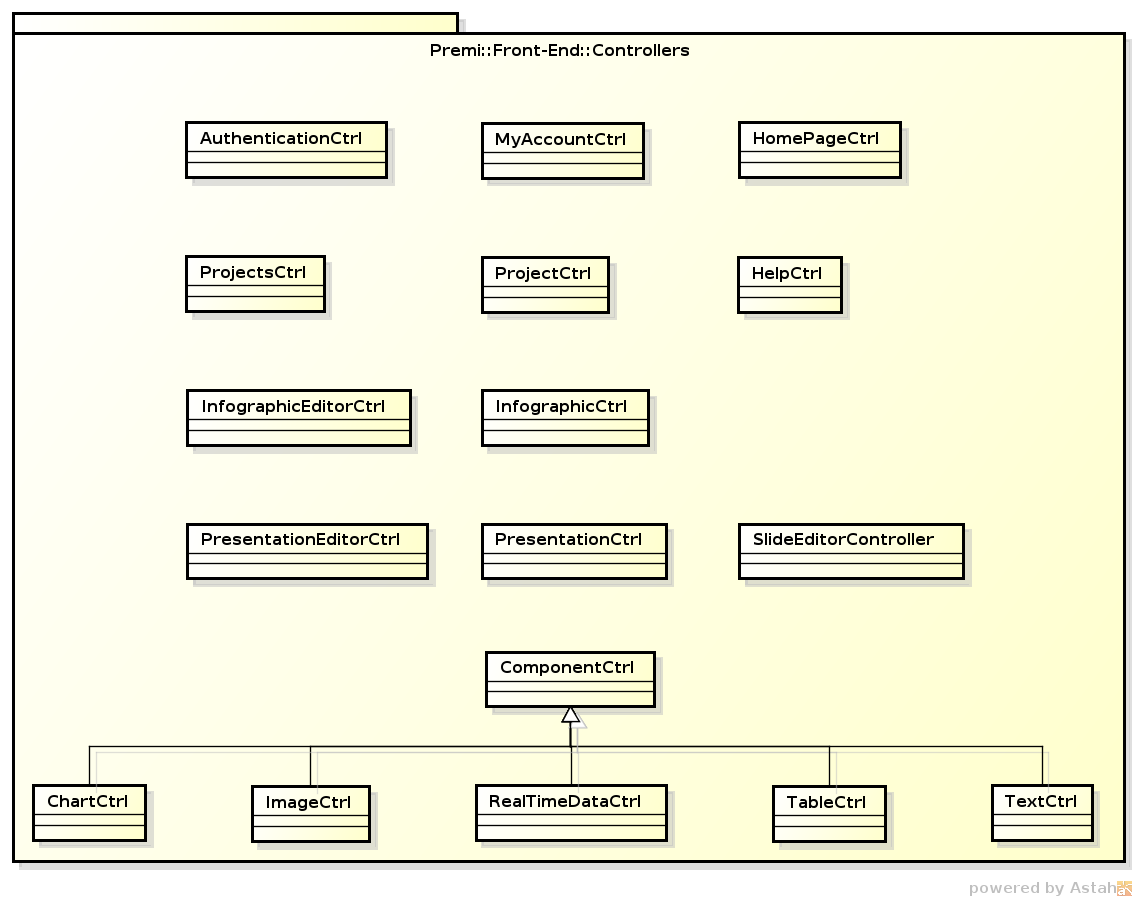
\includegraphics[width=1.0\linewidth]{img/premi_front_end_controllers}
	\caption[Premi::Front-End::Controllers]{Premi::Front-End::Controllers}
\end{figure}
Il package gestisce i controller del front-end dell'applicazione. Comunica con il model, le view e i service della struttura per gestire tutte le operazioni tra di essi. Fa comunicare le view con il model per rendere visibili gli aggiornamenti di quest'ultimo sulle view che utilizzano quei dati. Viceversa, aggiorna il model con le informazioni provenienti dalle view. Richiama inoltre i service per comunicare con il back-end rendendo possibile caricare o salvare i dati nel database.\\
Per brevità nell'identificare un controller è stata omessa la dicitura Premi::Front-End::Controllers lasciando solamente il nome del controller stesso. Si assume dunque che la dicitura compatta <nomeController> rappresenta la forma estesa Premi::Front-End::Controllers::<nomeController>.

\newpage
\subsubsection{AuthenticationCtrl}
\begin{figure}[h]
	\centering
	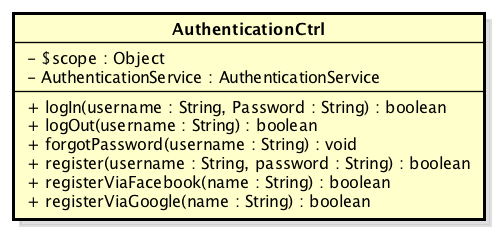
\includegraphics[width=0.5\linewidth]{img/premi_front_end_controllers_authenticationctrl}
	\caption[Premi::Front-End::Controllers::AuthenticationCtrl]{Premi::Front-End::Controllers::AuthenticationCtrl}
\end{figure}
\paragraph{Descrizione}
Il controller AuthenticationCtrl gestisce l'autenticazione di un utente nel sistema.

\paragraph{Utilizzo}
Questa classe viene utilizzata per gestire le richieste di autenticazione, disconnessione e gestione password all'interno del sistema e di regolare l'accesso alle aree riservate.
In particolare gestisce le operazioni di logIn, logOut e recupero Password.
\paragraph{Attributi}
\begin{itemize}
	\item \textbf{-\$scope: Object}:\\
	Campo dati contenente un riferimento all'oggetto \$scope creato da Angular, viene utilizzato come mezzo di comunicazione tra il controller e la view. Contiene gli oggetti che definiscono il model dell'applicazione.
	\item \textbf{-AuthenticationService: AuthenticationService}:\\
	Campo dati che contiene un riferimento al servizio che si occupa di gestire le funzionalità di autenticazione nel sistema.
\end{itemize}

\paragraph{Metodi}
\begin{itemize}
	\item \textbf{+logIn(\textit{username}:String, \textit{Password}:String):Boolean}:\\
	Metodo che permette di autenticare l'utente con username \textit{username} nel sistema verificando le sue credenziali;
	\item \textbf{+logOut(\textit{username}:String):Boolean}:\\
	Metodo che permette di disconnettere l'utente con username \textit{username} dal sistema restituendo \textit{true} in caso di successo e \textit{false} in caso di fallimento;
	\item \textbf{+forgotPassword(\textit{username}:String):void}:\\
	Metodo che si occupa di fornire il supporto al recupero password dell'utente con username \textit{username}.
	\item \textbf{+register(\textit{username}:String,\textit{password}:String):Boolean}:\\
	Metodo che esegue la procedura di registrazione di un nuovo utente con username \textit{username} e password \textit{password} restituendo \textit{true} in caso di successo e \textit{false} in caso di fallimento;
	\item \textbf{+registerViaFacebook(\textit{name}:String):Boolean}:\\
	Metodo che esegue la procedura di registrazione di un nuovo utente con le API di Facebook restituendo \textit{true} in caso di successo e \textit{false} in caso di fallimento;
	\item \textbf{+registerViaGooglePlus(\textit{name}:String):Boolean}:\\
	Metodo che esegue la procedura di registrazione di un nuovo utente con le API di Google+ restituendo \textit{true} in caso di successo e \textit{false} in caso di fallimento;
\end{itemize}
\paragraph{Relazioni con altre classi}
\begin{itemize}
	\item OUT: \textbf{Views::InfographicEditor}:\\
	La vista Views::InfographicEditor utilizza AuthenticationCtrl per autorizzare un utente alla composizione e modifica di una infografica;
	\item OUT: \textbf{Views::PresentationEditor}:\\
	La vista Views::PresentationEditor utilizza AuthenticationCtrl per autorizzare un utente alla composizione e modifica di una presentazione;
	\item OUT: \textbf{Views::SignUp}:\\
	La vista Views::SignUp utilizza AuthenticationCtrl per gestire permettere al sistema di registrare un nuovo utente;
	\item OUT: \textbf{Views::LogIn}:\\
	La vista Views::LogIn utilizza AuthenticationCtrl per gestire permettere ad un utente di accreditarsi nel sistema;
	\item OUT: \textbf{Views::Project}:\\
	La vista Views::Project utilizza AuthenticationCtrl per autorizzare un utente alla creazione e modifica di un progetto;
	\item IN: \textbf{AuthenticationService}:\\
	Il controller AuthenticationCtrl necessita di AuthenticationService per implementare la gestione delle autorizzazioni e modalità di connessione fornite agli utenti;
	
	\item IN: \textbf{Model::User}:\\
	Classe del model che gestisce gli utenti e le loro informazioni comprensive di quelle di autenticazione.
\end{itemize}

\newpage
\subsubsection{ChartCtrl}
\begin{figure}[h]
	\centering
	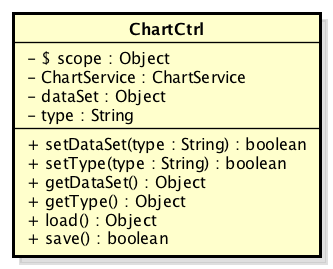
\includegraphics[width=0.4\linewidth]{img/premi_front_end_controllers_chartctrl}
	\caption[Premi::Front-End::Controllers::ChartCtrl]{Premi::Front-End::Controllers::ChartCtrl}
\end{figure}
\paragraph{Descrizione}
Il controller ChartCtrl concretizza ComponentCtrl e si occupa di fornire le primitive per la costruzione e gestione dei grafici in una slide.

\paragraph{Utilizzo}
Questa classe viene utilizzata per consentire all'utente di aggiungere, modificare o rimuovere un grafico in una slide.

\paragraph{Attributi}
\begin{itemize}
	\item \textbf{-\$scope: Object}:\\
	Campo dati contenente un riferimento all'oggetto \$scope creato da Angular, viene utilizzato come mezzo di comunicazione tra il controller e la view. Contiene gli oggetti che definiscono il model dell'applicazione;
	\item \textbf{-ChartService: ChartService}:\\
	\item\textbf{-dataSet:Object}:\\
	Array di oggetti JSON ognuno dei quali indica un dato da rappresentare nel grafico;
	\item\textbf{-type:String}:\\
	Campo dati che indica la tipologia di grafico da rappresentare.
\end{itemize}

\paragraph{Metodi}
\begin{itemize}
	\item \textbf{+setDataSet(\textit{type}:String):Boolean}:\\
	Metodo che permette di impostare i dati sorgente del grafico corrente restituendo \textit{true} in caso di successo e \textit{false} in caso di fallimento;
	\item \textbf{+setType(\textit{type}:String):Boolean}:\\
	Metodo che permette di impostare la tipologia di grafico restituendo \textit{true} in caso di successo e \textit{false} in caso di fallimento;
	\item \textbf{+getDataSet():Object}:\\
	Metodo che restituisce i dati sorgente del grafico corrente;
	\item \textbf{+getType():Object}:\\
	Metodo che restituisce la tipologia del grafico corrente.
	\item \textbf{+load():Object}:\\
	Metodo che permette di caricare un grafico proveniente dal server web dove risiede il sistema mediante l'utilizzo del servizio ChartService. Esso restituisce un oggetto JSON contenente la tipologia ed il set di dati del grafico in caso di successo ed una stringa vuota in caso di fallimento;
	\item \textbf{+save():Boolean}:\\
	Metodo che permette di salvare un grafico mediante l'utilizzo del servizio ChartService restituendo \textit{true} in caso di successo e \textit{false} in caso di fallimento.
	
\end{itemize}
\paragraph{Relazioni con altre classi}
\begin{itemize}
	\item IN: \textbf{ComponentCtrl}:\\
	Il controller ChartCtrl estende ComponentCtrl per la costruzione e gestione di grafici;
	\item IN: \textbf{ChartService}:\\
	Campo dati che contiene un riferimento al servizio che si occupa di gestire reperimento, cancellazione ed aggiornamento dei grafici all'interno del sistema;
	\item IN: \textbf{Model::Chart}:\\
	Il controller ChartCtrl utilizza Model::Chart per stabilire la struttura dell'oggetto che rappresenta;
	\item OUT: \textbf{SlideEditorCtrl}:\\
	Il controller SlideEditorCtrl necessita di ChartCtrl per la costruzione e gestione di grafici.
	
\end{itemize}

\newpage
\subsubsection{ComponentCtrl}
	\begin{figure}[h]
		\centering
		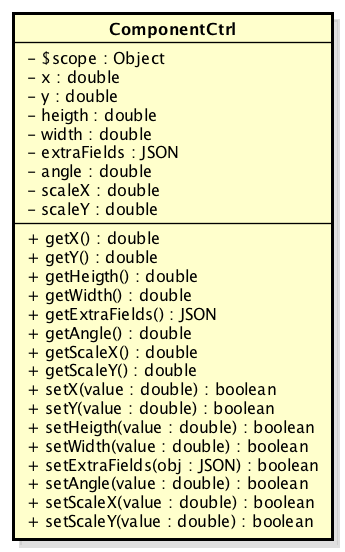
\includegraphics[width=0.4\linewidth]{img/premi_front_end_controllers_componentctrl}
		\caption[Premi::Front-End::Controllers::ComponentCtrl]{Premi::Front-End::Controllers::ComponentCtrl}
	\end{figure}

    \paragraph{Descrizione}
	Il controller ComponentCtrl si occupa di fornire le primitive per la costruzione e gestione dei componenti in una slide.\\
	È una classe astratta in quanto non sarà possibile istanziare un componente direttamente ma solo oggetti che concretizzano la classe costruendo oggetti dei tipi previsti dal sistema.\\

	\paragraph{Utilizzo}
	Questa classe viene utilizzata per consentire all'utente di aggiungere, modificare o rimuovere un componente in una slide.

	\paragraph{Attributi}
	\begin{itemize}
		\item \textbf{-\$scope: Object}:\\
			Campo dati contenente un riferimento all'oggetto \$scope creato da Angular, viene utilizzato come mezzo di comunicazione tra il controller e la view. Contiene gli oggetti che definiscono il model dell'applicazione;
		\item\textbf{-x:Double}:\\
			Campo dati contenente il valore della distanza dal bordo sinistro del canvas utilizzata per l'ancoraggio dell'oggetto;
		\item\textbf{-y:Double}:\\
			Campo dati contenente il valore della distanza dal bordo superiore del canvas utilizzata per l'ancoraggio dell'oggetto;
		\item\textbf{-heigth:Double}:\\
			Campo dati contenente il valore dell'altezza dell'oggetto;
		\item\textbf{-width:Double}:\\
			Campo dati contenente il valore della larghezza dell'oggetto;
		\item\textbf{-extraFields:Object}:\\
			Campo dati contenente eventuali parametri supplementari per ogni componente in un array di oggetti in formato JSON. Progettato in ottica di estensioni future;
		\item\textbf{-angle:Double}:\\
			Campo dati contenente il valore dell'angolo di rotazione;
		\item\textbf{-scaleX:Double}:\\
			Campo dati contenente il coefficiente di scala in orizzontale rispetto al valore originale rappresentato dal valore 1;
		\item\textbf{-scaleY:Double}:\\
			Campo dati contenente il coefficiente di scala in verticale rispetto al valore originale rappresentato dal valore 1.

	\end{itemize}

	\paragraph{Metodi}
	\begin{itemize}
	\item \textbf{+getX():Double}:\\
		Metodo che restituisce la distanza dal bordo sinistro del canvas utilizzata per l'ancoraggio dell'oggetto selezionato;
	\item \textbf{+getY():Double}:\\
		Metodo che restituisce la distanza dal bordo superiore del canvas utilizzata per l'ancoraggio dell'oggetto selezionato;
	\item \textbf{+getHeigth():Double}:\\
		Metodo che restituisce l'altezza dell'oggetto selezionato;
	\item \textbf{+getWidth():Double}:\\
		Metodo che restituisce la larghezza dell'oggetto selezionato;
	\item \textbf{+getExtraFields():JSON}:\\
		Metodo che restituisce un oggetto JSON con le informazioni aggiuntive dell'oggetto selezionato;
	\item \textbf{+getAngle():Double}:\\
		Metodo che restituisce l'angolo di rotazione dell'oggetto selezionato;
	\item \textbf{+getScaleX():Double}:\\
		Metodo che restituisce il livello di zoom applicato alla larghezza dell'oggetto selezionato;
	\item \textbf{+getScaleY():Double}:\\
		Metodo che restituisce il livello di zoom applicato all'altezza dell'oggetto selezionato;
	\item \textbf{+setX(\textit{value}:Double):Boolean}:\\
		Metodo che permette di impostare la distanza dal bordo sinistro del canvas utilizzata per l'ancoraggio dell'oggetto selezionato al valore \textit{value} restituendo \textit{true} in caso di successo e \textit{false} in caso di fallimento;
	\item \textbf{+setY(\textit{value}:Double):Boolean}:\\
		Metodo che permette di impostare la distanza dal bordo superiore del canvas utilizzata per l'ancoraggio dell'oggetto selezionato al valore \textit{value} restituendo \textit{true} in caso di successo e \textit{false} in caso di fallimento;
	\item \textbf{+setHeigth(\textit{value}:Double):Boolean}:\\
		Metodo che permette di impostare l'altezza dell'oggetto selezionato al valore \textit{value} restituendo \textit{true} in caso di successo e \textit{false} in caso di fallimento;
	\item \textbf{+setWidth(\textit{value}:Double):Boolean}:\\
		Metodo che permette di impostare la larghezza dell'oggetto selezionato al valore \textit{value} restituendo \textit{true} in caso di successo e \textit{false} in caso di fallimento;
	\item \textbf{+setExtraFields(\textit{obj}:JSON):Boolean}:\\
		Metodo che permette di impostare le proprietà aggiuntive dell'oggetto selezionato prendendo i valori dall'oggetto JSON \textit{obj} passato per parametro restituendo \textit{true} in caso di successo e \textit{false} in caso di fallimento;
	\item \textbf{+setAngle(\textit{value}:Double):Boolean}:\\
		Metodo che permette di impostare l'angolo di rotazione dell'oggetto selezionato al valore \textit{value} restituendo \textit{true} in caso di successo e \textit{false} in caso di fallimento;
	\item \textbf{+setScaleX(\textit{value}:Double):Boolean}:\\
		Metodo che permette di impostare il livello di zoom applicato alla larghezza dell'oggetto selezionato al valore \textit{value} restituendo \textit{true} in caso di successo e \textit{false} in caso di fallimento;
	\item \textbf{+setScaleY(\textit{value}:Double):Boolean}:\\
		Metodo che permette di impostare il livello di zoom applicato all'altezza dell'oggetto selezionato al valore \textit{value} restituendo \textit{true} in caso di successo e \textit{false} in caso di fallimento.
	\end{itemize}
	\paragraph{Relazioni con altre classi}
	\begin{itemize}

	 \item IN: \textbf{Model::Component}:\\
		Il controller ComponentCtrl utilizza Model::Component per stabilire la struttura dell'oggetto che rappresenta.
	 \item OUT: \textbf{SlideEditorCtrl}:\\
		Il controller SlideEditorCtrl utilizza ComponentCtrl per la gestione dei componenti al fine di costruire la slide.
	 \item OUT: \textbf{ChartCtrl}:\\
	 	Il controller ChartCtrl estende ComponentCtrl per la costruzione e gestione di grafici.
	 \item OUT: \textbf{ImageCtrl}:\\
		Il controller ImageCtrl estende ComponentCtrl per la costruzione e gestione di oggetti di tipo immagine.
	 \item OUT: \textbf{RealTimeDataCtrl}:\\
		Il controller RealTimeDataCtrl estende ComponentCtrl per la costruzione e gestione di oggetti con aggiornamento in tempo reale.
	 \item OUT: \textbf{TableCtrl}:\\
		Il controller TableCtrl estende ComponentCtrl per la costruzione e gestione di oggetti di tipo tabella.
	 \item OUT: \textbf{TextCtrl}:\\
		Il controller TextCtrl estende ComponentCtrl per la costruzione e gestione di oggetti di tipo testo.

	\end{itemize}

\newpage

\subsubsection{ImageCtrl}
\begin{figure}[h]
	\centering
	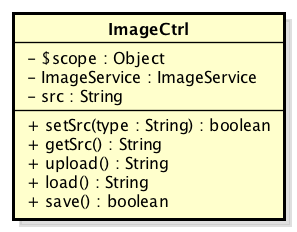
\includegraphics[width=0.4\linewidth]{img/premi_front_end_controllers_imagectrl}
	\caption[Premi::Front-End::Controllers::ImageCtrl]{Premi::Front-End::Controllers::ImageCtrl}
\end{figure}
   \paragraph{Descrizione}
	Il controller ImageCtrl concretizza ComponentCtrl e si occupa di fornire le primitive per la costruzione e gestione degli oggetti di tipo immagine all'interno di una slide.

	\paragraph{Utilizzo}
	Questa classe viene utilizzata per consentire all'utente di aggiungere, modificare o rimuovere un immagine in una slide.

	\paragraph{Attributi}
	\begin{itemize}
		\item \textbf{-\$scope: Object}:\\
			Campo dati contenente un riferimento all'oggetto \$scope creato da Angular, viene utilizzato come mezzo di comunicazione tra il controller e la view. Contiene gli oggetti che definiscono il model dell'applicazione;
		\item \textbf{-ImageService: ImageService}:\\
			Campo dati che contiene un riferimento al servizio che si occupa di gestire reperimento, cancellazione ed aggiornamento delle immagini all'interno del sistema.
		\item\textbf{-src:String}:\\
			Campo dati che indica il percorso dove è possibile recuperare l'immagine.
	\end{itemize}

	\paragraph{Metodi}
	\begin{itemize}
	\item \textbf{+setSrc(\textit{type}:String):Boolean}:\\
		Metodo che permette di impostare il percorso dove è possibile recuperare l'immagine restituendo \textit{true} in caso di successo e \textit{false} in caso di fallimento;
	\item \textbf{+getSrc():String}:\\
		Metodo che restituisce il percorso dove è possibile recuperare l'immagine.
	\item \textbf{+upload():String}:\\
		Metodo che permette di caricare un immagine proveniente da un dispositivo esterno al sistema restituendo il percorso dove risiede l'immagine in caso di successo ed una stringa vuota in caso di fallimento;
	\item \textbf{+load():String}:\\
		Metodo che permette di caricare una immagine proveniente dal server web dove risiede il sistema mediante l'utilizzo del servizio ImageService restituendo il percorso dell'immagine in caso di successo ed una stringa vuota in caso di fallimento;
	\item \textbf{+save():Boolean}:\\
		Metodo che permette di salvare una immagine mediante l'utilizzo del servizio ImageService restituendo \textit{true} in caso di successo e \textit{false} in caso di fallimento.
	\end{itemize}
	\paragraph{Relazioni con altre classi}
	\begin{itemize}
 	\item IN: \textbf{ComponentCtrl}:\\
	 	Il controller ImageCtrl estende ComponentCtrl per la costruzione e gestione di grafici;
	\item IN: \textbf{ImageService}:\\
		Il controller ImageCtrl necessita di ImageCtrl per il recupero ed il salvataggio delle immagini;
	\textbf{\item IN: \textbf{Model::Image}:\\
			Il controller ComponentCtrl utilizza Model::Image per stabilire la struttura dell'oggetto che rappresenta.}
	\item OUT: \textbf{SlideEditorCtrl}:\\
		Il controller SlideEditorCtrl necessita di ImageCtrl per la costruzione e gestione delle immagini.
	\end{itemize}

\newpage

\subsubsection{HelpCtrl}
\begin{figure}[h]
	\centering
	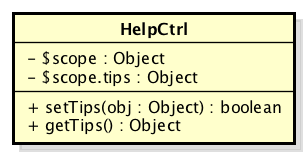
\includegraphics[width=0.4\linewidth]{img/premi_front_end_controllers_helpctrl}
	\caption[Premi::Front-End::Controllers::HelpCtrl]{Premi::Front-End::Controllers::HelpCtrl}
\end{figure}
      \paragraph{Descrizione}
	Il controller HelpCtrl gestisce i meccanismi di aiuto all'utente.

	\paragraph{Utilizzo}
	Questa classe viene utilizzata per gestire le informazioni e la logica di erogazione degli aiuti all'utente sotto forma di suggerimenti(tips) esplicativi delle funzionalità.

	\paragraph{Attributi}
	\begin{itemize}
		\item \textbf{-\$scope: Object}:\\
				Campo dati contenente un riferimento all'oggetto \$scope creato da Angular, viene utilizzato come mezzo di comunicazione tra il controller e la view. Contiene gli oggetti che definiscono il model dell'applicazione.
		\item \textbf{-\$scope.tips: Object}:\\
				Campo dati che racchiude in un array di oggetti JSON tutti i suggerimenti necessari allo svolgimento del tour tra le funzionalità del sistema ed al supporto all'utente.
	\end{itemize}

	\paragraph{Metodi}
	\begin{itemize}
	  \item \textbf{+setTips(\textit{obj}:Object):Boolean}:\\
		  Metodo che permette di aggiungere uno o più suggerimenti tramite un oggetto JSON. Il metodo restituisce \textit{true} in caso di successo e \textit{false} in caso di fallimento;
	  \item \textbf{+getTips():Object}:\\
		  Metodo che restituisce tutti i suggerimenti in un array di oggetti JSON in caso di successo ed un array vuoto in caso di fallimento.
	\end{itemize}
	\paragraph{Relazioni con altre classi}
	\begin{itemize}
	 \item OUT: \textbf{Views::SlideEditor}:\\
		La vista SlideEditorCtrl utilizza HelpCtrl per la gestione degli aiuti nella composizione e modifica di una slide.
	 \item OUT: \textbf{Views::InfographicEditor}:\\
		La vista Views::InfographicEditor utilizza HelpCtrl per la gestione degli aiuti nella composizione e modifica di una infografica.
	 \item OUT: \textbf{Views::Projects}:\\
		La vista Views::Projects utilizza HelpCtrl per la gestione degli aiuti nella gestione dei progetti dell'utente.
	 \item OUT: \textbf{Views::Search}:\\
		La vista SearchView utilizza HelpCtrl per la gestione degli aiuti nella ricerca di progetti.
	\end{itemize}

\newpage
\subsubsection{HomePageCtrl}
\begin{figure}[h]
	\centering
	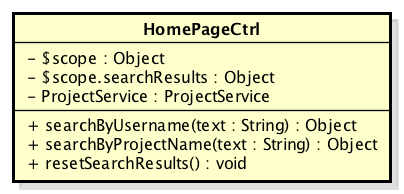
\includegraphics[width=0.5\linewidth]{img/premi_front_end_controllers_homepagectrl}
	\caption[Premi::Front-End::Controllers::HomePageCtrl]{Premi::Front-End::Controllers::HomePageCtrl}
\end{figure}
\paragraph{Descrizione}
Il controller HomePageCtrl gestisce gli strumenti messi a disposizione dalla Home Page. In particolare le funzionalità di ricerca.

\paragraph{Utilizzo}
Questa classe viene utilizzata per permettere alla vista Views::HomePage di riecrcare progetti per nome oppure per username dell'utente proprietario.\\
\paragraph{Attributi}
\begin{itemize}
	\item \textbf{-\$scope: Object}:\\
	Campo dati contenente un riferimento all'oggetto \$scope creato da Angular, viene utilizzato come mezzo di comunicazione tra il controller e la view. Contiene gli oggetti che definiscono il model dell'applicazione;
	\item \textbf{-\$scope.searchResults: Object}:\\
	Campo dati contenente le informazioni relative all'esito della ricerca;
	\item \textbf{-ProjectService: ProjectService}:\\
	Campo dati che contiene un riferimento al servizio che fornisce le funzionalità relative alla gestione di un progetto in aggiunta a quelle di ricerca.
	
\end{itemize}

\paragraph{Metodi}
\begin{itemize}
	\item \textbf{+\$scope.searchByUsername(\textit{text}:String):Object}:\\
	Metodo che recupera dal back-end le informazioni relative agli utenti che hanno una corrispondenza con la stringa mediante il service ProjectService::searchByUsernameService salvandole sull'oggetto \$scope.searchResults e restituendo un array di oggetti JSON con il suo contenuto;
	\item \textbf{+\$scope.searchByProjectName(\textit{text}:String):Object}:\\
	Metodo che recupera dal back-end le informazioni relative ai nomi di progetto che hanno una corrispondenza con la stringa mediante il service ProjectService::searchByProjectNameService salvandole sull'oggetto \$scope.searchResults e restituendo un array di oggetti JSON con il suo contenuto;
	\item \textbf{+\$scope.resetSearchResults():void}:\\
	Metodo che azzera i risultati di ricerca per poterne accogliere di nuovi oppure perché non più necessari.
	
\end{itemize}
\paragraph{Relazioni con altre classi}
\begin{itemize}
	\item OUT: \textbf{Views::HomePage}:\\
	La vista Views::HomePage utilizza HomePageCtrl per reperire ed aggiornare le informazioni di pertinenza dell'account relativo all'utente corrente;
	\item IN: \textbf{ProjectService}.
	La vista Views::HomePage utilizza il service ProjectService per recuperare ed aggiornare le informazioni relative ad un particolare progetto in aggiunta a quelle di ricerca.
\end{itemize}

\subsubsection{InfographicEditorCtrl}
\begin{figure}[h]
	\centering
	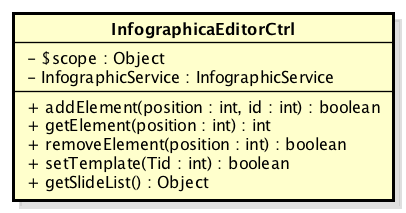
\includegraphics[width=0.4\linewidth]{img/premi_front_end_controllers_infographiceditorctrl}
	\caption[Premi::Front-End::Controllers::InfographicEditorCtrl]{Premi::Front-End::Controllers::InfographicEditorCtrl}
\end{figure}
	\paragraph{Descrizione}
		Il controller InfographicEditorCtrl gestisce la composizione e modifica di una infografica sulla base di template predefiniti che permettono l'inserimento in posizioni specifiche di slide precedentemente create.

	\paragraph{Utilizzo}

		Questa classe viene utilizzata per gestire le richieste da parte della vista InfographicEditor ed aggiornarla a seconda delle modifiche della classe Premi::Front-End::Model::Infographic.
		Ha il compito di tener traccia ed aggiornare codice identificativo e posizione delle slide in un template di infografica.
	\paragraph{Attributi}
	\begin{itemize}
		\item \textbf{-\$scope: Object}:\\
			Campo dati contenente un riferimento all'oggetto \$scope creato da Angular, viene utilizzato come mezzo di comunicazione tra il controller e la view. Contiene gli oggetti che definiscono il model dell'applicazione.
		\item \textbf{-InfographicService: InfographicService}:\\
			Campo dati che contiene un riferimento al servizio che si occupa di reperire e salvare le informazioni di una infografica.
	\end{itemize}

	\paragraph{Metodi}
	\begin{itemize}
	  \item \textbf{+addElement(\textit{position}:Int, \textit{id}:String):Boolean}:\\
		  Metodo che permette di aggiungere l'elemento con codice identificativo \textit{id} alla infografica in posizione \textit{position}.
	  \item \textbf{+getElement(\textit{position}:Int):String}:\\
		  Metodo che restituisce il codice identificativo dell'oggetto in posizione \textit{position} in caso di successo es una stringa vuota in caso di fallimento.
	  \item \textbf{+removeElement(\textit{position}:Int):Boolean}:\\
		  Metodo che elimina l'oggetto in posizione \textit{position} restituendo \textit{true} in caso di successo e \textit{false} in caso di fallimento.
	  \item \textbf{+setTemplate(\textit{Tid}:String):Boolean}:\\
		  Metodo che imposta il template \textit{Tid} per l'infografica corrente nella vista InfographicEditor restituendo \textit{true} in caso di successo e \textit{false} in caso di fallimento.
	  \item \textbf{+getSlideList():Object}:\\
		  Metodo che restituisce un oggetto JSON contenente un array con tutte le slide dell'infografica con le relative posizioni nel template.

	\end{itemize}
	\paragraph{Relazioni con altre classi}
	\begin{itemize}
		\item IN: \textbf{InfographicService}:\\
			Il controller InfographicCtrl necessita di InfographicService per il recupero ed il salvataggio delle informazioni necessarie alla corretta erogazione e gestione delle infografiche;
		\item OUT: \textbf{Views::InfographicEditor}:\\
			La vista InfographicEditor utilizza HelpCtrl per la gestione degli aiuti nella composizione e modifica di una infografica.
	\end{itemize}
\newpage


\subsubsection{MyAccountCtrl}
\begin{figure}[h]
	\centering
	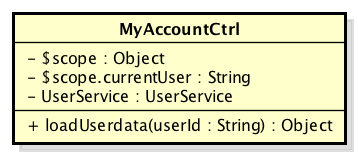
\includegraphics[width=0.4\linewidth]{img/premi_front_end_controllers_myaccountctrl}
	\caption[Premi::Front-End::Controllers::MyAccountCtrl]{Premi::Front-End::Controllers::MyAccountCtrl}
\end{figure}
\paragraph{Descrizione}
Il controller MyAccountCtrl gestisce le funzionalità di visualizzazione e modifica di un profilo utente.

\paragraph{Utilizzo}
Questa classe viene utilizzata per permettere alla vista Views::SlideEditor di inserire componenti in un a slide, modificarne le caratteristiche oppure eliminarli.\\
\paragraph{Attributi}
\begin{itemize}
	\item \textbf{-\$scope: Object}:\\
	Campo dati contenente un riferimento all'oggetto \$scope creato da Angular, viene utilizzato come mezzo di comunicazione tra il controller e la view. Contiene gli oggetti che definiscono il model dell'applicazione;
	\item \textbf{-\$scope.currentUser: String}:\\
	Campo dati contenente le informazioni relative all'utente correntemente collegato al sistema;
	\item \textbf{-UserService: UserService}:\\
	Campo dati che contiene un riferimento al servizio che fornisce le funzionalità relative alla gestione di un utente.
\end{itemize}

\paragraph{Metodi}
\begin{itemize}
	\item \textbf{+loadUserdata(\textit{userId}:String):Object}:\\
	Metodo che recupera dal back-end le informazioni relative all'utente identificato da \textit{id} mediante il service UserService salvandole sull'oggetto \$scope.currentUser e restituendo un oggetto JSON con il suo contenuto.
\end{itemize}
\paragraph{Relazioni con altre classi}
\begin{itemize}
	\item OUT: \textbf{Views::MyAccount}:\\
	La vista Views::MyAccount utilizza MyAccountCtrl per reperire ed aggiornare le informazioni di pertinenza dell'account relativo all'utente corrente;
	\item IN: \textbf{UserService}.
	La vista Views::MyAccount utilizza il service UserService per recuperare ed aggiornare le informazioni relative ad un particolare utente.
	
\end{itemize}

\newpage
\subsubsection{PresentationCtrl}
\begin{figure}[h]
	\centering
	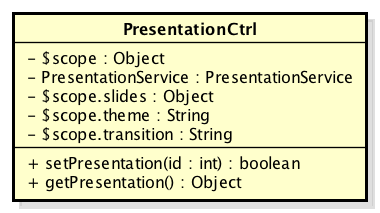
\includegraphics[width=0.4\linewidth]{img/premi_front_end_controllers_presentationctrl}
	\caption[Premi::Front-End::Controllers::PresentationCtrl]{Premi::Front-End::Controllers::PresentationCtrl}
\end{figure}
	\paragraph{Descrizione}
	Il controller PresentationCtrl gestisce la creazione e visualizzazione di una presentazione.

	\paragraph{Utilizzo}
	Questa classe viene utilizzata per gestire le richieste da parte della vista Views::Presentation ed aggiornarla a seconda delle modifiche della classe Premi::Front-End::Model::Presentation. PresentationCtrl ha la responsabilità di rendere persistenti le modifiche di un progetto nel front-end anche nel back-end mediante una chiamata al servizio PresentationService.
	Ha il compito di tener traccia delle slide da visualizzare e delle rispettive posizioni\footnote{La presentazione è organizzata secondo una griglia, quindi per ogni slide è necessario salvare le coordinate X e Y.}.
	\paragraph{Attributi}
	\begin{itemize}
		\item \textbf{-\$scope: Object}:\\
			Campo dati contenente un riferimento all'oggetto \$scope creato da Angular, viene utilizzato come mezzo di comunicazione tra il controller e la view. Contiene gli oggetti che definiscono il model dell'applicazione;
		\item \textbf{-PresentationService: PresentationService}:\\
			Campo dati che contiene un riferimento al servizio che si occupa di reperire le informazioni necessarie alla vista Views::Presentation e di fornire le funzionalità necessarie alla corretta erogazione della presentazione;
		\item \textbf{-\$scope.slides: Object}:\\
			Campo dati che contiene sottoforma di array di oggetti JSON tutte le slide appartenenti alla presentazione. Ogni slide è corredata dalle coordinate cartesiane di posizionamento sulla griglia;

		\item \textbf{-\$scope.theme: String}:\\
			Campo dati che contiene un riferimento alla configurazione grafica che l'utente ha scelto come predefinita per la sua presentazione;

		\item \textbf{-\$scope.transition: String}:\\
			Campo dati che contiene un riferimento alla tipologia di transizione tra slide che l'utente ha scelto come predefinita per la sua presentazione.
	\end{itemize}

	\paragraph{Metodi}
	\begin{itemize}
	  \item \textbf{+setPresentation(\textit{id}:String):Boolean}:\\
		  Metodo che imposta la presentazione identificata da  \textit{id} per la corretta erogazione da parte della vista Views::Presentation restituendo \textit{true} in caso di successo e \textit{false} in caso di fallimento;
	  \item \textbf{+getPresentation():Object}:\\
		  Metodo che restituisce un array di oggetti JSON contenente un array con tutte le slides della presentazione con le relative coordinate nella presentazione corrente.

	\end{itemize}
	\paragraph{Relazioni con altre classi}
	\begin{itemize}
	  \item OUT: \textbf{Views::Presentation}:\\
		La vista Views::Presentation utilizza PresentationCtrl per la gestione e visualizzazione di una presentazione;
	  \item IN: \textbf{PresentationService}: \\
	  	Il servizio PresentationService viene utilizzato per il reperimento ed il salvataggio di una presentazione.
	\end{itemize}

\newpage
\subsubsection{PresentationEditorCtrl}
\begin{figure}[h]
	\centering
	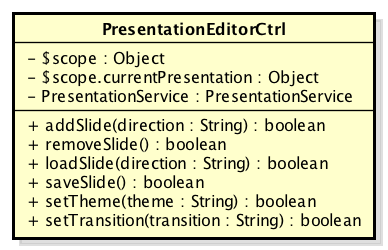
\includegraphics[width=0.5\linewidth]{img/premi_front_end_controllers_presentationeditorctrl}
	\caption[Premi::Front-End::Controllers::PresentationEditorCtrl]{Premi::Front-End::Controllers::PresentationEditorCtrl}
\end{figure}

	\paragraph{Descrizione}
	Il controller PresentationEditorCtrl si occupa della modifica di una presentazione con i metodi per gestire le slide.

	\paragraph{Utilizzo}
	Questa classe viene utilizzata per consentire all'utente di aggiungere o rimuovere una slide dalla presentazione in una posizione qualsiasi e spostarsi tra di esse. Permette inoltre di impostare lo stile e il template della presentazione.

	\paragraph{Attributi}
	\begin{itemize}
		\item \textbf{- PresentationService: PresentationService}:\\
			Campo dati che contiene un riferimento al servizio che si occupa della gestione dei dati e delle impostazioni di una presentazione;
		\item \textbf{- \$scope: Object}:\\
			Campo dati contenente un riferimento all'oggetto \$scope creato da Angular, viene utilizzato come mezzo di comunicazione tra il controller e la view. Contiene gli oggetti che definiscono il model dell'applicazione.
		\item \textbf{- \$scope.currentPresentation: Object}:\\
			Campo dati che contiene un array di oggetti JSON contenenti le informazioni della presentazione corrente;

	\end{itemize}

	\paragraph{Metodi}
	\begin{itemize}
		\item \textbf{addSlide(direction: String):Boolean}:\\
			Metodo che aggiunge una slide alla presentazione rispetto alla slide corrente nella posizione indicata da \textit{direction}\footnote{Per \textit{direction} si intende la direzione nella quale si vuole aggiungere o caricare una slide\{up, right, down, left\}}. Il metodo restituisce \textit{true} in caso di successo e \textit{false} in caso di fallimento;
		\item \textbf{removeSlide():Boolean}:\\
			Metodo che rimuove la slide corrente dal canvas di modifica restituendo \textit{true} in caso di successo e \textit{false} in caso di fallimento;
		\item \textbf{loadSlide(direction: String):Boolean}\\
			Metodo che carica la slide nella posizione indicata da \textit{direction} nel canvas di modifica restituendo \textit{true} in caso di successo e \textit{false} in caso di fallimento;
		\item \textbf{saveSlide():Boolean}\\
			Metodo che salva la slide correntemente caricata sul canvas di modifica restituendo \textit{true} in caso di successo e \textit{false} in caso di fallimento;
		\item \textbf{setTheme(theme: String):Boolean}
			Metodo che imposta l'aspetto grafico predefinito per la presentazione al valore passato per parametro restituendo \textit{true} in caso di successo e \textit{false} in caso di fallimento;
		\item \textbf{setTransition(transition: String):Boolean}
			Metodo che imposta lo stile di transizione tra slide al valore passato per parametro restituendo \textit{true} in caso di successo e \textit{false} in caso di fallimento.
	\end{itemize}
	\paragraph{Relazioni con altre classi}
	\begin{itemize}
	  \item OUT: \textbf{Views::PresentationEditor}:\\
		La vista Views::PresentationEditor utilizza PresentationEditorCtrl per la gestione delle slide nella composizione e modifica di una presentazione;
	  \item IN: \textbf{PresentationService}:\\
	  	Il controller PresentationEditorCtrl utilizza il servizio PresentationService per il recupero ed il salvataggio di una presentazione interagendo con il back-end;
	  \item IN: \textbf{SlideEditorCtrl}:\\
	  	Il controller SlideEditorCtrl utilizza PresentationEditorCtrl per ottenere ed agguiornare le informazioni sul progetto corrente.
	\end{itemize}

\newpage


\subsubsection{ProjectCtrl}
\begin{figure}[h]
	\centering
	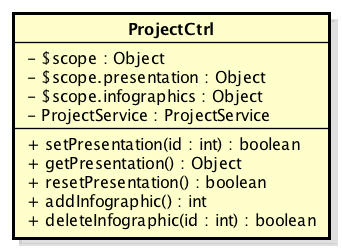
\includegraphics[width=0.4\linewidth]{img/premi_front_end_controllers_projectctrl}
	\caption[Premi::Front-End::Controllers::ProjectCtrl]{Premi::Front-End::Controllers::ProjectCtrl}
\end{figure}
	\paragraph{Descrizione}
	Il controller ProjectCtrl gestisce il progetto corrente.

	\paragraph{Utilizzo}
	Questa classe viene utilizzata per modificare un progetto esistente\footnote{Un progetto vuoto viene creato di default con una presentazione vuota.}.\\
	Permette di aggiungere infografiche, richiamare le funzionalità di modifica di infografiche e della presentazione. Inoltre permette di lanciare la vista di visualizzazione della presentazione.
	\paragraph{Attributi}
	\begin{itemize}
		\item \textbf{-\$scope: Object}:\\
			Campo dati contenente un riferimento all'oggetto \$scope creato da Angular, viene utilizzato come mezzo di comunicazione tra il controller e la view. Contiene gli oggetti che definiscono il model dell'applicazione;
		\item \textbf{-\$scope.presentation: Object}:\\
			Campo dati contenente un riferimento alla presentazione appartenente al progetto corrente;
		\item \textbf{-\$scope.infographics: Object}:\\
			Campo dati contenente un array di oggetti JSON ognuno rappresentante una infografica del progetto corrente;
		\item \textbf{-ProjectService: ProjectService}:\\
			Campo dati che contiene un riferimento al servizio che si occupa di reperire le informazioni necessarie al corretto funzionamento della vista Views::Project.
	\end{itemize}

	\paragraph{Metodi}
	\begin{itemize}
	  	\item \textbf{+setPresentation(\textit{id}:String):Boolean}:\\
		  	Metodo che imposta la presentazione identificata da  \textit{id} per la corretta erogazione della presentazione da parte della vista Views::Presentation restituendo \textit{true} in caso di successo e \textit{false} in caso di fallimento;
	  	\item \textbf{+getPresentation():Object}:\\
		  	Metodo che restituisce un oggetto JSON contenente un array con tutte le slide della presentazione con le relative coordinate nella presentazione;
	 	\item \textbf{+resetPresentation():Boolean}:\\
			Metodo che riporta la presentazione relativa al progetto corrente allo stato iniziale ovvero dotata di una sola slide vuota restituendo \textit{true} in caso di successo e \textit{false} in caso di fallimento;
		\item \textbf{+addInfographic():String}:\\
			Metodo che inserisce ua nuova infografica al progetto corrente restituendone il codice identificativo;
		\item \textbf{+deleteInfographic(\textit{id}:String):Boolean}:\\
	  		Metodo che elimina l'infografica identificata da \textit{id} dal progetto corrente restituendo \textit{true} in caso di successo e \textit{false} in caso di fallimento.


	\end{itemize}
	\paragraph{Relazioni con altre classi}
	\begin{itemize}
	  \item OUT: \textbf{Views::Project}:\\
		La vista Views::Project utilizza ProjectCtrl per la gestione reperire ed aggiornare le informazioni di pertinenza del progetto corrente;
	  \item IN: \textbf{ProjectService}.
		La vista Views::Project utilizza il service ProjectService per reperire ed aggiornare le informazioni di pertinenza del progetto corrente dal back-end.
	\end{itemize}

\newpage
\subsubsection{ProjectsCtrl}
\begin{figure}[h]
	\centering
	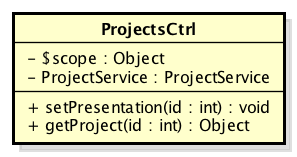
\includegraphics[width=0.4\linewidth]{img/premi_front_end_controllers_projectsctrl}
	\caption[Premi::Front-End::Controllers::ProjectsCtrl]{Premi::Front-End::Controllers::ProjectsCtrl}
\end{figure}
	\paragraph{Descrizione}
	Il controller ProjectsCtrl gestisce i progetti dell' utente corrente.

	\paragraph{Utilizzo}
	Questa classe viene utilizzata per visualizzare tutti i progetti dell'utente corrente, lanciarne la modalità di modifica (gestita da ProjectCtrl) e crearne di nuovi.\\
	\paragraph{Attributi}
	\begin{itemize}
		\item \textbf{-\$scope: Object}:\\
			Campo dati contenente un riferimento all'oggetto \$scope creato da Angular, viene utilizzato come mezzo di comunicazione tra il controller e la view. Contiene gli oggetti che definiscono il model dell'applicazione;
		\item \textbf{-ProjectService: ProjectService}
	\end{itemize}

	\paragraph{Metodi}
	\begin{itemize}
	  \item \textbf{+setPresentation(\textit{id}:String):void}:\\
		  Metodo che imposta la presentazione identificata da  \textit{id} per la corretta erogazione della presentazione da parte della vista Views::Presentation;
	  \item \textbf{+getProject(\textit{id}:String):Object}:\\
		  Metodo che restituisce un oggetto JSON contenente un array con la presentazione e tutte le infografiche del progetto identificato da \textit{id}.

	\end{itemize}
	\paragraph{Relazioni con altre classi}
	\begin{itemize}
	  \item OUT: \textbf{Views::Projects}:\\
		La vista Views::Projects utilizza ProjectsCtrl per la gestione reperire ed aggiornare le informazioni di pertinenza dei progetti dell'utente corrente;
	  \item IN: \textbf{ProjectService}.
		La vista Views::Projects utilizza il service ProjectService per reperire ed aggiornare le informazioni di pertinenza dei progetti dell'utente corrente dal back-end.
	\end{itemize}

\newpage

\subsubsection{RealTimeDataCtrl}
\begin{figure}[h]
	\centering
	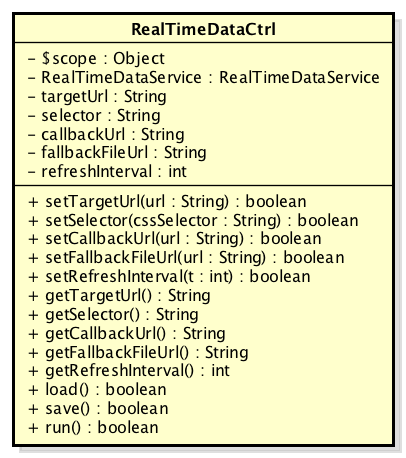
\includegraphics[width=0.5\linewidth]{img/premi_front_end_controllers_realtimedatactrl}
	\caption[Premi::Front-End::Controllers::RealTimeDataCtrl]{Premi::Front-End::Controllers::RealTimeDataCtrl}
\end{figure}
\paragraph{Descrizione}
Il controller RealTimeDataCtrl concretizza ComponentCtrl e si occupa di fornire le primitive per la costruzione e gestione degli oggetti di tipo immagine all'interno di una slide.

\paragraph{Utilizzo}
Questa classe viene utilizzata per consentire all'utente di aggiungere, modificare o rimuovere delle componenti con aggiornamento periodico all'interno di una slide.

\paragraph{Attributi}
\begin{itemize}
	\item \textbf{-\$scope: Object}:\\
	Campo dati contenente un riferimento all'oggetto \$scope creato da Angular, viene utilizzato come mezzo di comunicazione tra il controller e la view. Contiene gli oggetti che definiscono il model dell'applicazione;
	\item \textbf{RealTimeDataService:RealTimeDataService}:\\
	Campo dati che contiene un riferimento al servizio che si occupa di gestire reperimento, cancellazione ed aggiornamento dei dati in tempo reale all'interno del sistema;
	\item \textbf{-targetUrl:String}:\\
	Campo dati che indica il percorso dove è possibile recuperare le informazioni;
	\item \textbf{-selector:String}:\\
	Campo dati che indica il selettore, secondo le regole del css, dove individuare i dati di interesse all'interno dell'indirizzo contenuto in targetUrl;
	\item \textbf{-callbackUrl:String}:\\
	Campo dati che indica l'indirizzo dove reperire il file in formato javascript che ha il compito di elaborare ed impaginare i dati ottenuti in precedenza;
	\item \textbf{-fallbackFileUrl:String}:\\
	Campo dati che indica il percorso dove trovare le informazioni in caso di impossibilità di raggiungere la risorsa;
	\item \textbf{-refreshInterval: Int}:\\
	Campo dati che indica il tempo che intercorre tra gli aggiornamenti dei dati in secondi.
	
\end{itemize}

\paragraph{Metodi}
\begin{itemize}
	\item \textbf{+setTargetUrl(\textit{url}:String):Boolean}:\\
	Metodo che permette di impostare il percorso della risorsa che contiene le informazioni d'interesse restituendo \textit{true} in caso di successo e \textit{false} in caso di fallimento;
	\item \textbf{+setSelector(\textit{cssSelector}:String):Boolean}:\\
	Metodo che permette di impostare il selettore all'interno del targetUrl che permette di raggiungere le informazioni d'interesse al valore \textit{cssSelector}, restituendo \textit{true} in caso di successo e \textit{false} in caso di fallimento;
	\item \textbf{+setCallbackUrl(\textit{url}:String):Boolean}:\\
	Metodo che permette di impostare il percorso della risorsa che contiene le informazioni d'interesse restituendo \textit{true} in caso di successo e \textit{false} in caso di fallimento;
	\item \textbf{+setFallbackFileUrl(\textit{url}:String):Boolean}:\\
	Metodo che permette di impostare il percorso dove trovare le informazioni in caso di impossibilità di reperire la risorsa d'interesse al valore \textit{url}, restituendo \textit{true} in caso di successo e \textit{false} in caso di fallimento;
	\item \textbf{+setRefreshInterval(\textit{t}:Int):Boolean}:\\
	Metodo che permette di impostare il tempo che intercorre tra due aggiornamenti successivi al valore di \textit{t} secondi, restituendo \textit{true} in caso di successo e \textit{false} in caso di fallimento;
	\item \textbf{+getTargetUrl():String}:\\
	Metodo che restituisce il percorso della risorsa che contiene le informazioni d'interesse;
	\item \textbf{+getSelector():String}:\\
	Metodo che restituisce il selettore all'interno del targetUrl che permette di raggiungere le informazioni d'interesse;
	\item \textbf{+getCallbackUrl():String}:\\
	Metodo che restituisce il percorso della risorsa che contiene le informazioni d'interesse;
	\item \textbf{+getFallbackFileUrl():String}:\\
	Metodo che restituisce il percorso dove reperire le informazioni in caso di impossibilità di raggiungere la risorsa d'interesse;
	\item \textbf{+getRefreshInterval():Int}:\\
	Metodo che restituisce il tempo che intercorre tra due aggiornamenti successivi del componente d'interesse;
	\item \textbf{+load():Boolean}:\\
	Metodo che permette di reperire le informazioni del componente dal file di fallback, ove presente, ed istanziare il componente, prescindendo dalla raggiungibilità o meno della risorsa mediante l'utilizzo del servizio RealTimeService. Viene restituito \textit{true} in caso di successo e \textit{false} in caso di fallimento;
	\item \textbf{+save():Boolean}:\\
	Metodo che permette di aggiornare le informazioni del componente nel file di fallback, ove presente, ed istanziare il componente mediante l'utilizzo del servizio RealTimeDataService. Viene restituito \textit{true} in caso di successo e \textit{false} in caso di fallimento;
	\item \textbf{+run():Boolean}:\\
	Metodo che permette di eseguire tutte le chiamate che provocano l'ottenimento del codice html finale da aggiornare nella slide mediante l'utilizzo del servizio RealTimeDataService restituendo \textit{true} in caso di successo e \textit{false} in caso di fallimento.
	Nello specifico le operazioni svolte sono le seguenti:
	\begin{enumerate}
		\item Viene scaricato il contenuto della risorsa referenziata da targetUrl. Se non è disponibile, il sistema riproverà l'operazione automaticamente facendo tre tentativi attendendo di volta in volta per trenta secondi. In caso di ulteriore fallimento sarà necessario un aggiornamento della pagina per la corretta erogazione di questa attività;
		\item Viene recuperata l'informazione d'interesse mediante il selettore;
		\item Viene processato l'output del passaggio precedente mediante uno script presente nel file disponibile all'indirizzo callbackUrl restituendo del codice html;
		\item Vengono salvate le informazioni del punto precente nel file di fallback mediante il metodo save;
		\item Viene aggiornato il contenuto della slide.
	\end{enumerate}
	
\end{itemize}
\paragraph{Relazioni con altre classi}
\begin{itemize}
	\item IN: \textbf{ComponentCtrl}:\\
	Il controller RealTimeDataCtrl estende ComponentCtrl per la costruzione e gestione di componenti con aggiornamento in tempo reale;
	\item IN: \textbf{RealTimeDataService}:\\
	Il controller RealTimeDataCtrl necessita di RealTimeDataService per il recupero ed il salvataggio delle informazioni necessarie alla corretta erogazione e gestione degli oggetti con aggiornamento in tempo reale;
	\item IN: \textbf{Model::RealTimeData}:\\
	Il controller RealTimeDataCtrl utilizza Model::RealTimeData per stabilire la struttura dell'oggetto che rappresenta;
	
	\item OUT: \textbf{SlideEditorCtrl}:\\
	Il controller SlideEditorCtrl necessita di ComponentCtrl per la costruzione e gestione degli oggetti con aggiornamento in tempo reale.
\end{itemize}

\newpage


\subsubsection{SlideEditorCtrl}
\begin{figure}[h]
	\centering
	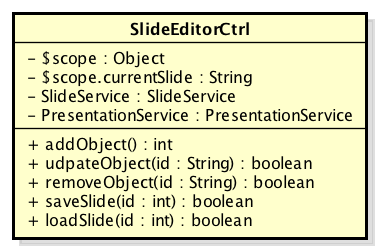
\includegraphics[width=0.5\linewidth]{img/premi_front_end_controllers_slideeditorctrl}
	\caption[Premi::Front-End::Controllers::SlideEditorCtrl]{Premi::Front-End::Controllers::SlideEditorCtrl}
\end{figure}
	\paragraph{Descrizione}
	Il controller SlideEditorCtrl gestisce le funzionalità di modifica di una slide.

	\paragraph{Utilizzo}
	Questa classe viene utilizzata per permettere alla vista Views::SlideEditor di inserire componenti in un a slide, modificarne le caratteristiche oppure eliminarli.\\
	\paragraph{Attributi}
	\begin{itemize}
		\item \textbf{-\$scope: Object}:\\
			Campo dati contenente un riferimento all'oggetto \$scope creato da Angular, viene utilizzato come mezzo di comunicazione tra il controller e la view. Contiene gli oggetti che definiscono il model dell'applicazione;
		\item \textbf{-\$scope.currentSlide:String}:\\
			Campo dati contenente le informazioni relative alla slide correntemente gestita dall'editor;
		\item \textbf{-SlideService: SlideService}:\\
			Campo dati che contiene un riferimento al servizio che si occupa di gestire le funzionalità di modifica e gestione di una slide.
		\item \textbf{-PresentationService: PresentationService}:\\
			Campo dati che contiene un riferimento al servizio che si occupa di gestire le funzionalità di modifica e gestione di una Presentazione.
	\end{itemize}

	\paragraph{Metodi}
	\begin{itemize}
	  \item \textbf{+addObject():String}:\\
		 Metodo che esegue la procedura di aggiunta di un nuovo componente nella slide corrente mediante una chiamata al service PresentationService ritornando il codice identificativo \textit{id}.
	  \item \textbf{+udpateObject(\textit{id}:String):Boolean}:\\
		 Metodo che esegue la procedura di aggiornamento di un componente  identificato da \textit{id} nella slide corrente mediante una chiamata al service PresentationService  restituendo \textit{true} in caso di successo e \textit{false} in caso di fallimento.\\I valori sono reperiti dalla variabile \$scope.selectedObject;
	  \item \textbf{+removeObject(\textit{id}:String):Boolean}\\
		 Metodo che esegue la rimozione del componente identificato da \textit{id} nella slide corrente mediante una chiamata al service SlideService  restituendo \textit{true} in caso di successo e \textit{false} in caso di fallimento.
	  \item \textbf{+saveSlide(\textit{id}:String):Boolean}:\\
		 Metodo che esegue la procedura di salvataggio della slide corrente mediante una chiamata al service SlideService restituendo \textit{true} in caso di successo e \textit{false} in caso di fallimento.
	  \item \textbf{+loadSlide(\textit{id}:String):Boolean}:\\
		 Metodo che esegue la procedura di caricamento della slide corrente sulla variabile \$scope.currentSlide mediante una chiamata al service PresentationService restituendo \textit{true} in caso di successo e \textit{false} in caso di fallimento.

	\end{itemize}
	\paragraph{Relazioni con altre classi}
	\begin{itemize}
	  \item OUT: \textbf{Views::SlideEditor}:\\
		La vista Views::SlideEditor utilizza SlideEditorCtrl per reperire ed aggiornare le informazioni di pertinenza della slide corrente;
	  \item IN: \textbf{SlideService}:\\
		Il controller SlideEditorCtrl utilizza il service SlideService per recuperare ed aggiornare le informazioni relative ad una particolare slide;
	  \item IN: \textbf{PresentationEditorCtrl}:\\
		Il controller SlideEditorCtrl utilizza  PresentationEditorCtrl per la gestione delle slide nella presentazione corrente.

	\item IN: \textbf{ChartCtrl}:\\
		Il controller SlideEditorCtrl necessita di ChartCtrl per la costruzione e gestione di grafici nella slide corrente;
	\item IN: \textbf{ImageCtrl}:\\
		Il controller SlideEditorCtrl necessita di ImageCtrl per la costruzione e gestione delle immagini nella slide corrente.
	\item IN: \textbf{RealTimeDataCtrl}:\\
		Il controller SlideEditorCtrl necessita di RealTimeDataCtrl per la costruzione e gestione di dati aggiornati in tempo reale nella slide corrente;
	\item IN: \textbf{TableCtrl}:\\
		Il controller SlideEditorCtrl necessita di TableCtrl per la costruzione e gestione delle tabelle nella slide corrente;
	\item IN: \textbf{TextCtrl}:\\
		Il controller SlideEditorCtrl necessita di TextCtrl per la costruzione e gestione di componenti di tipo testuale nella slide corrente.
	\end{itemize}

\newpage


\subsubsection{TableCtrl}
\begin{figure}[h]
	\centering
	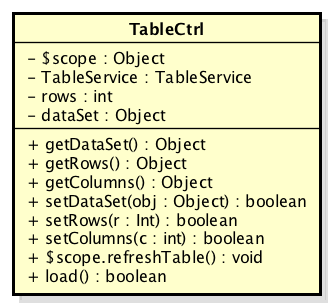
\includegraphics[width=0.4\linewidth]{img/premi_front_end_controllers_tablectrl}
	\caption[Premi::Front-End::Controllers::TableCtrl]{Premi::Front-End::Controllers::TableCtrl}
\end{figure}
\paragraph{Descrizione}
Il controller TableCtrl concretizza ComponentCtrl e si occupa di fornire le primitive per la costruzione e gestione degli oggetti di tipo tabella all'interno di una slide.

\paragraph{Utilizzo}
Questa classe viene utilizzata per consentire all'utente di aggiungere, modificare o rimuovere tabelle in una slide.

\paragraph{Attributi}
\begin{itemize}
	\item \textbf{-\$scope: Object}:\\
	Campo dati contenente un riferimento all'oggetto \$scope creato da AngularJs, viene utilizzato come mezzo di comunicazione tra il controller e la view. Contiene gli oggetti che definiscono il model dell'applicazione;
	\item  \textbf{-TableService:TableService}:\\
	Campo dati che contiene un riferimento al servizio che si occupa di gestire reperimento, cancellazione ed aggiornamento delle immagini all'interno del sistema.
	\item\textbf{-rows:int}:\\
	Campo dati che indica il numeri di righe che compongono la tabella.
	\item\textbf{-columns:int}:\\
	Campo dati che indica il numeri di colonne che compongono la tabella.
	\item\textbf{-dataSet:Object}:\\
	Array di oggetti JSON ognuno dei quali indica un dato da rappresentare nel grafico comprensivo di coordinate;
\end{itemize}

\paragraph{Metodi}
\begin{itemize}
	\item \textbf{+getDataSet():Object}:\\
	Metodo che restituisce i dati sorgente della tabella corrente;
	\item \textbf{+getRows():Object}:\\
	Metodo che restituisce il numero di righe della tabella corrente;
	\item \textbf{+getColumns():Object}:\\
	Metodo che restituisce il numero di colonne della tabella corrente;
	\item \textbf{+setDataSet(\textit{obj}:Object):Boolean}:\\
	Metodo che permette di impostare i dati sorgentedella tabella corrente al valore \textit{obj} restituendo \textit{true} in caso di successo e \textit{false} in caso di fallimento;
	\item \textbf{+setRows(\textit{r}:Int):Boolean}:\\
	Metodo che restituisce il numero di righe della tabella corrente  al valore \textit{r} restituendo \textit{true} in caso di successo e \textit{false} in caso di fallimento;
	\item \textbf{+setColumns(\textit{c}:Int):Boolean}:\\
	Metodo che restituisce il numero di colonne della tabella corrente \textit{c} restituendo \textit{true} in caso di successo e \textit{false} in caso di fallimento;
	\item \textbf{+\$scope.refreshTable():void}:\\
	Metodo che ridisegna la tabella d'interesse;
	\item \textbf{+load():Boolean}:\\
	Metodo che permette di caricare le informazioni relative alla tabella corrente mediante l'utilizzo del servizio TableService che produce un array di oggetti JSON \textit{"A"} in output. La tabella verrà poi aggiornata invocando il metodo setDataSet(\textit{"A"}) restituendo \textit{true} in caso di successo e \textit{false} in caso di fallimento;
	
\end{itemize}
\paragraph{Relazioni con altre classi}
\begin{itemize}
	\item IN: \textbf{ComponentCtrl}:\\
	Il controller TableCtrl estende ComponentCtrl per la costruzione e gestione di tabelle;
	\item IN: \textbf{TableService}:\\
	Il controller TableCtrl necessita di TableService per la gestione, il recupero ed il salvataggio delle tabelle;
	\item IN: \textbf{Model::Table}:\\
	Il controller TableCtrl utilizza Model::Table per stabilire la struttura dell'oggetto che rappresenta;
	\item OUT: \textbf{SlideEditorCtrl}:\\
	Il controller SlideEditorCtrl necessita di TableCtrl per la costruzione e gestione delle tabelle.
\end{itemize}

\newpage
\subsubsection{TextCtrl}
\begin{figure}[h]
	\centering
	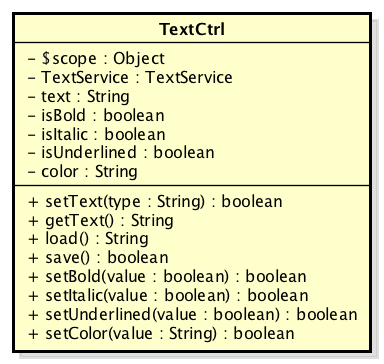
\includegraphics[width=0.4\linewidth]{img/premi_front_end_controllers_textctrl}
	\caption[Premi::Front-End::Controllers::TextCtrl]{Premi::Front-End::Controllers::TextCtrl}
\end{figure}
\paragraph{Descrizione}
Il controller TextCtrl concretizza ComponentCtrl e si occupa di fornire le primitive per la costruzione e gestione degli oggetti di tipo testuale all'interno di una slide.

\paragraph{Utilizzo}
Questa classe viene utilizzata per consentire all'utente di aggiungere, modificare o rimuovere un testo in una slide.

\paragraph{Attributi}
\begin{itemize}
	\item \textbf{-\$scope: Object}:\\
	Campo dati contenente un riferimento all'oggetto \$scope creato da Angular, viene utilizzato come mezzo di comunicazione tra il controller e la view. Contiene gli oggetti che definiscono il model dell'applicazione;
	\item  \textbf{TextService:TextService}\\
	Campo dati che contiene un riferimento al servizio che si occupa di gestire reperimento, cancellazione ed aggiornamento dei componenti di tipo testuale all'interno del sistema.
	\item\textbf{-text:String}:\\
	Campo dati che indica la stringa di testo da rappresentare.
	\item\textbf{-isBold:Boolean}:\\
	Campo dati che, con valore true, indica che il testo deve essere rappresentato in grassetto; È stato scelto \textit{false} come valore di default;
	\item\textbf{-isItalic:Boolean}:\\
	Campo dati che, con valore true, indica che il testo deve essere rappresentato in corsivo; È stato scelto \textit{false} come valore di default;
	\item\textbf{-isUnderlined:Boolean}:\\
	Campo dati che, con valore true, indica che il testo deve essere rappresentato con una sottolineatura. È stato scelto \textit{false} come valore di default;
	\item\textbf{-color:String}:\\
	Campo dati che indica il colore del testo utilizzando un cancelletto seguito da sei caratteri esadecimali. La prima coppia rappresenta la percentuale di rosso, la seconda di verde e la terza di blu con i range così determinati:
	\begin{itemize}
		\item '00' = 0\%;
		\item 'FF' = 100\%.
	\end{itemize}
	È stato previsto il nero (\#000000) come colore predefinito per il testo.
	
	
\end{itemize}

\paragraph{Metodi}
\begin{itemize}
	\item \textbf{+setText(\textit{type}:String):Boolean}:\\
	Metodo che permette di impostare la stringa di testo da rappresentare restituendo \textit{true} in caso di successo e \textit{false} in caso di fallimento;
	\item \textbf{+getText():String}:\\
	Metodo che restituisce il contenuto testuale dell'oggetto corrente situato nella variabile \$scope.text.
	\item \textbf{+load():String}:\\
	Metodo che permette di caricare un componente testuale mediante l'utilizzo del servizio TextService restituendo l'oggetto Object corrispondente in caso di successo ed un oggetto vuoto in caso di fallimento.
	\item \textbf{+save():Boolean}:\\
	Metodo che permette di salvare un componente testuale mediante l'utilizzo del servizio TextService restituendo \textit{true} in caso di successo e \textit{false} in caso di fallimento;
	\item \textbf{+setBold(\textit{value}:Boolean):Boolean};
	Metodo che permette di im postare la proprietà "grassetto" dell'oggetto testuale corrente al valore \textit{value} restituendo \textit{true} in caso di successo e \textit{false} in caso di fallimento;
	\item \textbf{+setItalic(\textit{value}:Boolean):Boolean};
	Metodo che permette di im postare la proprietà "corsivo" dell'oggetto testuale corrente al valore \textit{value} restituendo \textit{true} in caso di successo e \textit{false} in caso di fallimento;
	\item \textbf{+setUnderlined(\textit{value}:Boolean):Boolean};
	Metodo che permette di im postare la proprietà "sottolineato" dell'oggetto testuale corrente al valore \textit{value} restituendo \textit{true} in caso di successo e \textit{false} in caso di fallimento;
	\item \textbf{+setColor(\textit{value}:String):Boolean};
	Metodo che permette di im postare il colore dell'oggetto testuale corrente al valore \textit{value} restituendo \textit{true} in caso di successo e \textit{false} in caso di fallimento.
	
\end{itemize}
\paragraph{Relazioni con altre classi}
\begin{itemize}
	\item IN: \textbf{TextCtrl}:\\
	Il controller TextCtrl estende ComponentCtrl per la costruzione e gestione di componenti testuali.
	\item IN: \textbf{TextService}:\\
	Il controller TextCtrl necessita di TextService per il recupero ed il salvataggio delle informazioni necessarie alla corretta erogazione e gestione degli oggetti di tipo testuale;
	\item IN: \textbf{Model::Text}:\\
	Il controller TextCtrl utilizza Model::Text per stabilire la struttura dell'oggetto che rappresenta;
	\item OUT: \textbf{SlideEditorCtrl}:\\
	Il controller SlideEditorCtrl necessita di TextCtrl per la costruzione e gestione di componenti testuali.
\end{itemize}

\newpage

